\chapter{Propozycja klasyfikatorów}
\section{Klasyfikator ekspercki}
Klasyfikator ekspercki powstał na bazie doświadczeń z podstawowymi klasyfikatorami. W zależności o charakterystyki danych, osiągana skuteczność przez klasyfikatory może się różnić. Klasyfikator skutecznie rozpoznający klasy jednego zbioru, może miernie klasyfikować inny zbiór, podczas gdy użycie innego klasyfikatora na tym samym zbiorze danych może znacząco poprawić osiągane wyniki. Również użycie różnych algorytmów klasyfikacji, połączenie ich w komitet może zmniejszyć błąd klasyfikacji. 
Klasyfikator ekspercki został stworzony w celu zmniejszenia błędu klasyfikacji niezależnie od typu danych oraz nieznanych danych. \par
\begin{figure}[h]
	\centering
	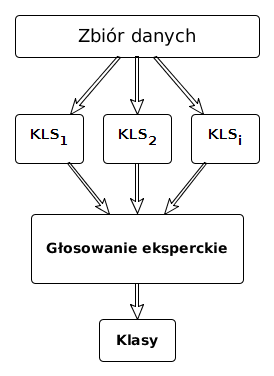
\includegraphics[width=\textwidth]{./images/klas_ekspercki.png}
	\caption{Schemat klasyfikatora eksperckiego. $KB_1..KB_i$ to klasyfikatory bazowe.}
	\label{fig:klasyfikator_ekspercki}
\end{figure}
Klasyfikator ekspercki to połączenie kilku klasyfikatorów bazowych (przynajmniej trzech). Każdy klasyfikator trenowany jest na zbiorze uczącym, a następnie oceniana jest jakość klasyfikacji każdego z osobna. Stworzono dwie wersje klasyfikatora, w pierwszej klasyfikator uczony i testowany jest na tym samym zbiorze danych, w drugiej oceniany jest z wykorzystaniem sprawdzianu krzyżowego (domyślnie k=3). W kolejnym etapie, dla każdej klasy wyłaniany jest klasyfikator ekspert. Ekspert klasowy wybierany jest na podstawie najwyższego współczynnika dla danej klasy. Tworząc klasyfikator można wybrać na podstawie którego współczynnika precyzji, F1 czy G-mean będą wyłaniani eksperci. Domyślnie jest to współczynnik precyzji. Przy wyborze miary G-mean ekspert dla obu będzie taki sam. Jeżeli ocena odbywała się ze sprawdzianem krzyżowym, to modele bazowe tworzone są od nowa na całym zbiorze treningowym. \par
W procesie klasyfikacji właściwej nowych próbek, najpierw klasyfikowane są przez klasyfikatory bazowe. Końcowa klasa wyznaczana jest według algorytmu:
\begin{enumerate}
	\item Jeżeli występuje zgodność co do klasy pomiędzy klasyfikatorami to wybierana jest ta klasa.
	\item Jeżeli tylko jeden ekspert wskaże swoją klasę to ostateczną klasą jest ta wskazana przez eksperta.
	\item Jeżeli dwóch ekspertów wskażą swoje klasy, to wybierana jest klasa z większym prawdopodobieństwem wskazanym przez klasyfikator. W przypadku takich samych prawdopodobieństw, wybierana jest klasa wskazana przez klasyfikator z większym współczynnikiem G-mean.
	\item Jeżeli żaden ekspert nie wskaże swojej klasy, to klasa wybierana jest poprzez głosowanie większościowe
\end{enumerate}
\subsection{Testy}

\section{Meta-klasyfikator}

\begin{figure}[H]
	\centering
	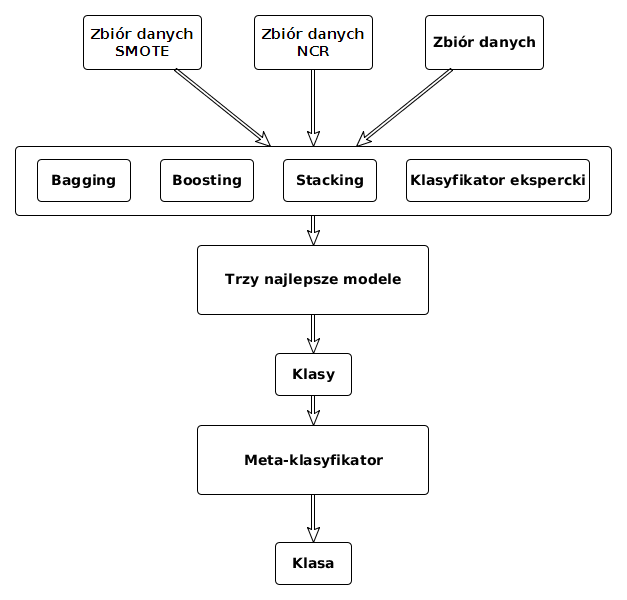
\includegraphics[width=\textwidth]{./images/metaklas.png}
	\caption{Projekt meta klasyfikatora}
	\label{fig:metaklasmoj}
\end{figure}
\subsection{Testy}